%%%%%%%%%%%%%%%%%%%%%%%%%%%%%%%%%%%%%%%%%%%%%%%%%%%%%%%%%%%%%%%%%%%%%%%%%%%%%%%%%%%%%%%%%%%%%%%%%%%%%%%%%%%%%%%%%%%%%%%%%%%%%%%%%%%%%%%%%
% Abstract: dar uma idéia dos principais resultados encontrados. 
% Introdução: cenário, motivacao, problema, solucoes atuais, escopo do artigo, lista de contribuicoes, organizacao do resto do artigo. 
% Trabalhos Relacionados: fazer uma das duas coisas a seguir (ou as duas): 
%	a) quando citar uma ou um grupo de referencias relacionado an um tema especifico, conclua o paragrafo mostrando a diferenca para a proposta a ser descrita. 
%	b) no final da secao, compile todas as diferenças e deixe explicito as contribuicoes novamente.
% Metodologia: coloque uma figura para ilustrar todo o processo de coleta e analise. coloque numa tabela (ou mais de uma) a descricao das metricas de interesse, alem dos fatores e niveis selecionados em outra tabela. explique o motivo desses fatores influenciarem as metricas de interesse.
% Conclusão: evite apresentar os resultados mais fáceis de concluir. bons revisores olham o casamento do que vc escreve no abstract/introdução com a conclusao, então mantenha coerente an introdução com a conclusão. Em geral, resultados que sao aparentemente obvios - nao eram até vc mostrar :) - enfraquecem as outras contribuicoes. p.ex, "Os resultados mostraram que o MapReduce apresenta uma boa solução para utilizar computadores comuns para obter alta capacidade de processamento e lidar com an análise massiva de tráfego de rede." pode ser reformulado ou retirado da conclusao. 
\chapter{Eigensim for Anomaly Detection in Offline Mobile Client}
\label{ch:3_mobile}


The protection scheme used in a mobile device should be both computationally secure as well as resource-constrained due to battery power limitations \cite{khan2015cloud}. Therefore, encrypting files and generating keys on a mobile device is not considered a good solution. On the other hand, the protection schemes with good computational qualities lack the security analysis in many cases \cite{khan2014bss}. The common practice is the shadow user activities monitoring \cite{yovel2014}. However, the mobile device usage stays unprotected in all the proposed scenarios while in offline mode. When the mobile client goes offline with the sensitive corporate data on board all powerful cloud-based tools can not help and the mobile client has to secure itself with its own limited resources. Moreover, due to the resources constraint, there is a crucial difference in strategy of online and offline mode protection.

Additional security issues and requirements have to be considered when mobile clients are actively used in corporate cloud environment \cite{yovel2014}. Today more and more organizations and enterprises are functioning in the Bring-Your-Own-Device (BYOD) paradigm. The uncontrolled usage of the mobile devices represents a serious risk to the development of secure SME cloud platforms being the bottleneck of the corporate information security system (ISS). While the enterprise cloud infrastructure based on the web interface can be protected by powerful third-party services, such as CASB and CAC, the corporate mobile client is usually light-weighted and generally less protected. 

This work proposes an architecture and approach for user behavior analysis based on Eigensim \cite{vieira2017model}, in order to detect possible threats in offline corporate mobile applications. The key expiration period is safely incorporated into the proposed system solution in order to enhance security and the behavioral analysis can indicate malicious behaviors, their variations, as well as novel attacks, which present low or high variance in comparison to legitimate user behaviors.

The work is structured as follows. Section \ref{sec:3_related_works} analyzes the most common security problems in the mobile cloud environment and the solutions for offline protection in the BYOD world. Section \ref{sec:3_the_client_security_architecture} outlines the mobile security architecture of the proposed solution. Section \ref{sec:3_offline_mode} presents the detailed scheme of the proposed solution to the problem of offline mobile client security. Section \ref{sec:3_eigensim} explains the use of Eigensim. Section \ref{sec:3_results} discusses the common threat scenarios, the data modeling, the performance analysis and discussion of the practical implementation results. Section \ref{sec:3_conclusion} concludes the chapter.


\section{Related works}
\label{sec:3_related_works}

The increasing usage of BYOD demands more sophisticated data protection services compared to ordinary computing environment. A common practice is to provide additional contextual methods apart from authentication, DLP services, and encryption, which can be at rest, in transit and in use \cite{yovel2014, khan2015cloud, khan2014survey, khan2013towards}. The contextual methods increase the security of the mobile client at a maximum level with minimum resource requirements. The most commonly used are:

\begin{enumerate}
	\item Using geolocation of the device to trace its usage;
	\item Setting up the expiration period of an app;
	\item Setting up the expiration period of client pass pin;
	\item Setting up the counter of failed tries;
	\item Secured transfer politics between apps;
	\item Restricting access to the corporate app;
	\item Restricted or prohibited offline access;
	\item Logging and auditing.
\end{enumerate}

Preventing data leakage on the mobile device is a crucial security problem. Therefore, it is necessary to take additional control and protection measures for the confidential data on the mobile devices that leave the boundaries of the organization. Generally, the most sensitive and confidential data should not be permitted to be transferred to the mobile device. However, what if the SME need to allow their employees to work on such devices and even use them on the offline mode for the convenience and traffic reducing, or even for a particular characteristic of the mobile client or the business itself?

From the theoretical point of view of this problem, there are several surveys, whose common point is the mobile cloud as a rapidly developing paradigm that poses many security and complexity problems \cite{khan2013towards, yovel2014, khan2014survey, khan2015cloud, mayrhofer2015architecture, chang2015design, xia2015tinman, kulkarni2015addressing, shila2016amcloud, heydari2016efficient}. Kulkarni and Khanai \cite{kulkarni2015addressing} discuss the most important threats related to Mobile Cloud Computing and argue that there is a need for a lightweight secure framework that provides security with minimum communication and processing overhead on mobile devices. 

An analysis of the new models of mobile cloud computing and new ways of using data storage services is presented in \cite{khan2015cloud, khan2013towards, mayrhofer2015architecture, chang2015design}. Commonly, the models and protection schemes concentrate on the encryption properties and either perform the computations on their own \cite{zhao2010trusted, yang2011provable} or use the cloud provider to off-load the cryptographic operations \cite{itani2010energy, ren2011lightweight}. Obviously, it is natural the mobile client cannot handle all operations securely without the assistance of a cloud provider, due to resources constraint and battery limitation.

The necessity to use schemes that function without putting load on a provider arises when it is desired to make the mobile client less dependent on the cloud provider, i.e. corporate client continues to provide the secure access to the sensitive data without connection to the network. As discussed in \cite{khan2015cloud}, all the currently known schemes of encryption, performing the computation, either use a cloud provider \cite{zhao2010trusted}, a third party trusted agent \cite{yang2011provable, heydari2016efficient}, a combination of both \cite{itani2010energy} or ad hoc approaches \cite{shila2016amcloud}. In some cases, they concentrate on computational complexity without taking care of user privacy and security \cite{ren2011lightweight}. Therefore, according to \cite{khan2013towards, khan2015cloud}, the state-of-the-art mobile cloud security models do not consider the problem of the offline security mode. 

To the best of our knowledge, the offline mode security problem has not yet been deployed, neither in academia nor in the industry \cite{yovel2014, khan2015cloud, khan2014survey, khan2013towards}. Therefore, the main concern of this proposal is the protection of the mobile client and its data in offline mode, when the functions of data protection cannot be offloaded to a cloud or a trusted party. 

\section{The mobile security architecture}
\label{sec:3_the_client_security_architecture}

The approach proposed in this work describes and implements a mobile client security infrastructure for malicious behavior analysis. The mobile security processes depend on the key expiry period, and are used to access the protected storage. Once the user keys expire, the user is requested to enter his valid credentials, i.e. PIN and password. The mobile client then sends the credentials to the server for verification. Once the new set of access keys is received, the user can access the protected files in the offline mode, without the access to the server. This means that no further communication with the server is needed until the key expires. 

The core set of functions and protocols of the proposed architecture can be divided into three sets of operations as shown in Figure \ref{fig:3_01}.

\begin{figure}[h!]
	\centering
	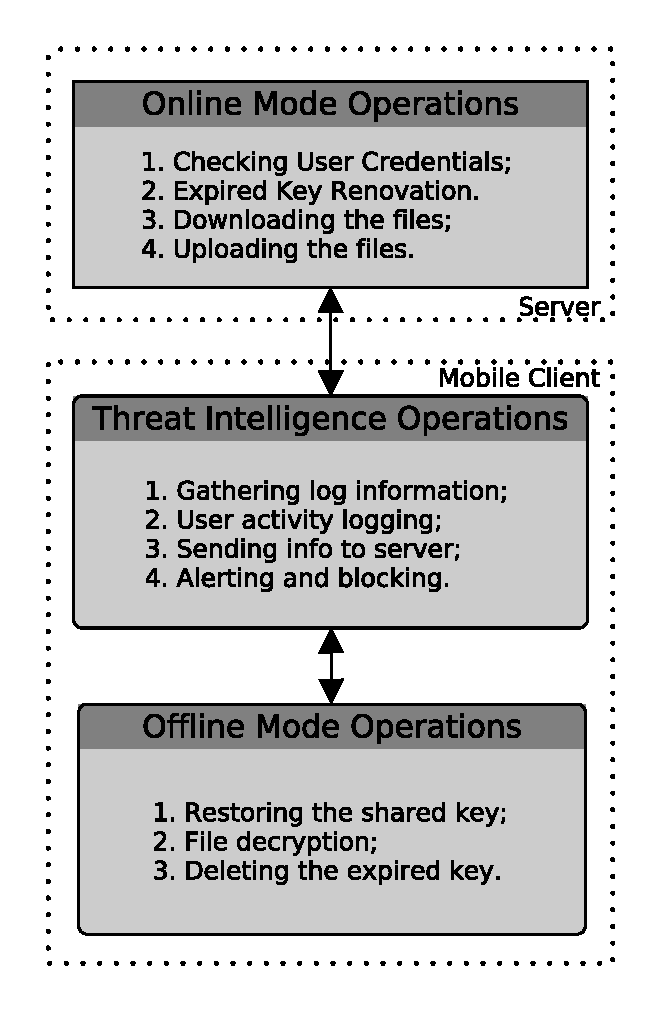
\includegraphics[width=8cm]{figs/ch3/fig01.eps}
	\caption{The core set of functions and protocols of the mobile cloud security infrastructure}
	\label{fig:3_01}
\end{figure}

Figure \ref{fig:3_01} describes the mobile client protection both in online and offline mode. In online mode, the client has the possibility to connect to the server and the security of the client is enhanced by the server-backed up mechanisms. On the other hand, in offline mode the client’s security is supported by the standalone mechanisms. Additionally, the mobile client protection is enhanced by the threat intelligence unit providing the constant monitoring and analysis.

Figure \ref{fig:3_02} depicts the client-side protection mechanisms. The client should support 4 subsystems: 
\begin{enumerate}
	\item Encryption subsystem that provides the procedures of encryption and decryption;
	\item Protected storage subsystem that provides the downloaded shares and key storage protection;
	\item The Threat intelligence unit that provides the constant monitoring;
	\item The communication subsystem that enables with the server.
\end{enumerate}

In summary, all security procedures are connected to 4 groups of operations: file request and receiving; encryption and decryption; file and key storing; monitoring and analysis.

\begin{figure}[h!]
	\centering
	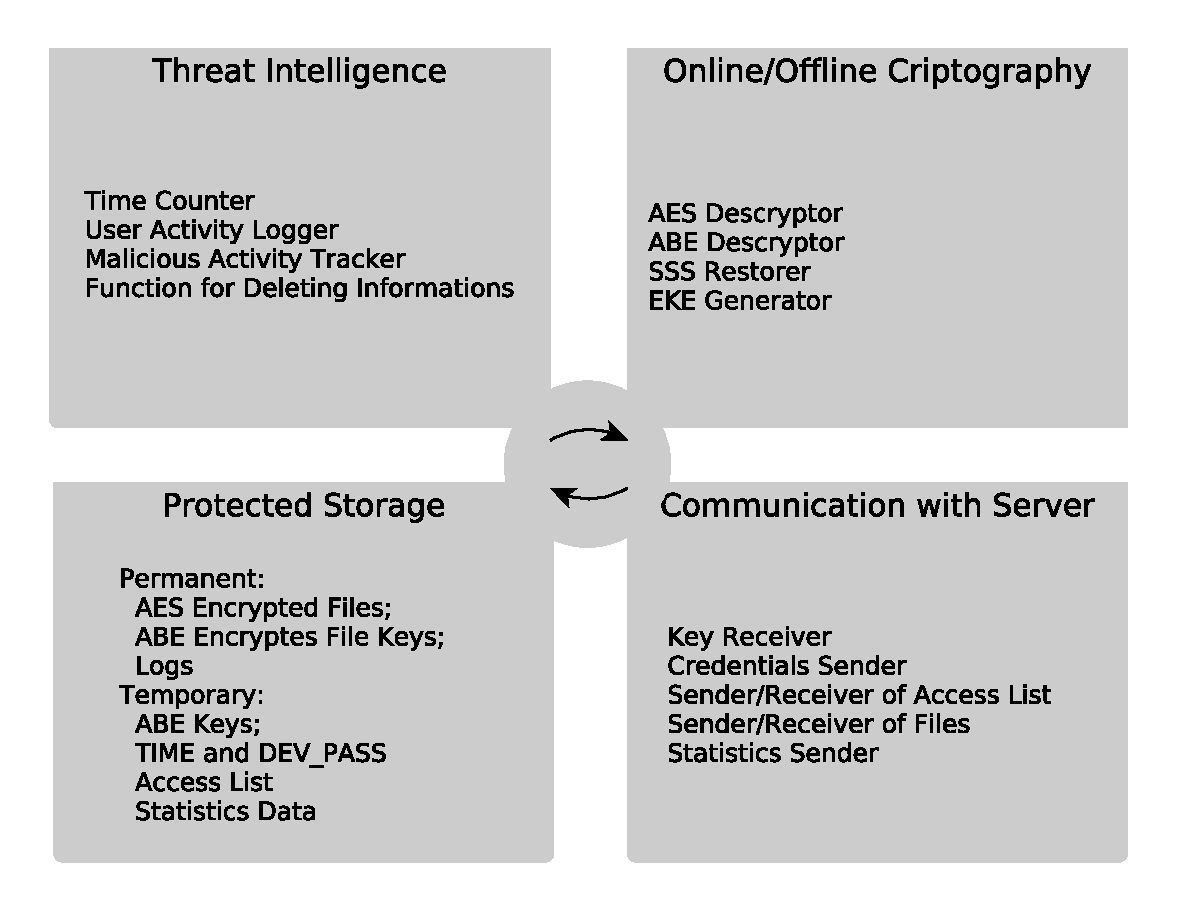
\includegraphics[width=12cm]{figs/ch3/fig02.eps}
	\caption{The Client-side Architecture}
	\label{fig:3_02}
\end{figure}

This architecture consists of the modules of cryptographic functions, threat intelligence infrastructure, communication with server and storage. However, this work focus on the threat intelligence infrastructure module for malicious behavior analysis.

The threat intelligence infrastructure takes into account simple actors such as the time counter for the key expiry period, the counter of unsuccessful tries in order to protect from brute force attacks, and Eigensim-inspired statistics analyzer. Functions such as alerting and deleting the expired key belong to this module as well. These functions are described in Subsection \ref{sec:3_eigensim}.

\section{The proposed solution for offline mobile security}
\label{sec:3_offline_mode}

This section proposes an approach for the mobile client protection in which the security is supported in offline modes. Currently and to the best of our knowledge, the systems of mobile client protection follow a model where the protected client can operate only when it is connected to the cloud, which is not always convenient for the end-user. The basic principles of the mobile client protection herein proposed are: 

\begin{enumerate}
	\item Optimized communication with the cloud when the mobile client does not need to be constantly connected to the server due to the resource constraint and necessity to secure this communication;
	\item Optimized combination of the security mechanisms so that the mobile client does not need to perform complex computation like encryption and key generation due to its resource constraint;
	\item Behavioral analysis of user's operations on mobile client, which can indicate anomalous or automated activities performed by attackers.
\end{enumerate}

The most important security issues in the proposed model arise when the client goes to the offline mode and the user is still allowed to get the access to the protected SME documents. In this case, the server can neither monitor the user activity nor provide the protection methods. The security should be performed at the mobile client. Additionally, the maximum protection should be provided at the minimum resource cost. 

In the online mode the mobile client uses the secure communication with the server in order to verify the validity of user’s credentials. On the contrary, the offline protection model should be approached independently.

\begin{figure}[h!]
	\centering
	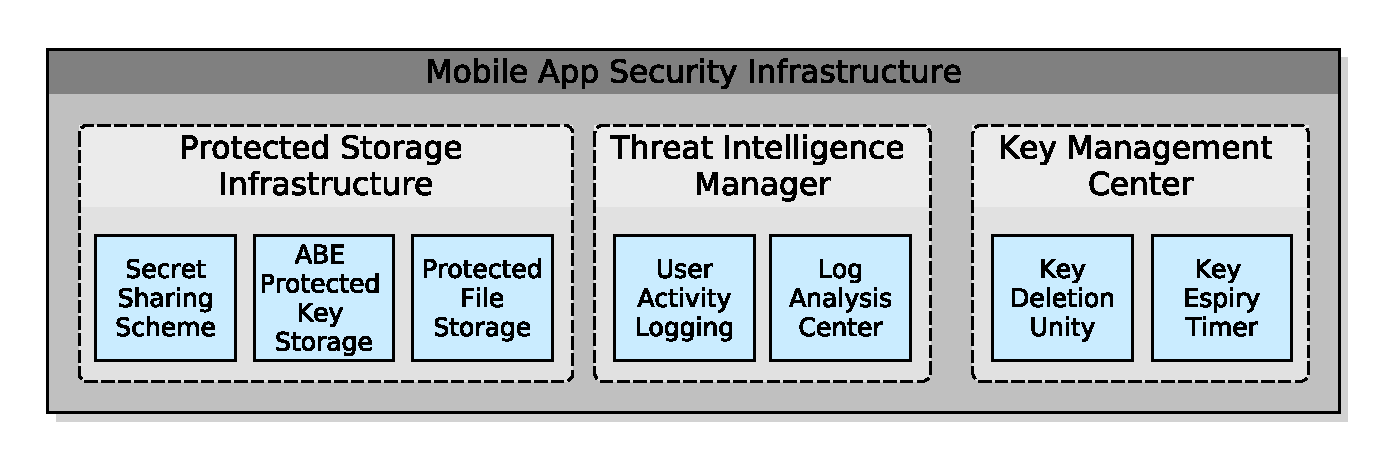
\includegraphics[width=15cm]{figs/ch3/fig03.eps}
	\caption{Proposed Architecture for Offline Mobile Security}
	\label{fig:3_03}
\end{figure}

The Figure \ref{fig:3_03} describes the proposed architecture for offline mobile security, showing the modules responsible for securing the mobile client, which includes:

\begin{enumerate}
	\item \pmb{Protected Storage}: the storage is protected with the shared user key and contains the ABE keys giving access to the file keys which allow decrypting the stored files.
	\item \pmb{Threat Intelligence Manager (TIM)}: most attacks incur into significant variation on the legitimate behavior of information systems, or they adopt well-known patterns that can be easily detected by monitoring the system in the case of the offline mode. Signal processing techniques have been successfully applied to anomaly detection \cite{lu2009network, huang2009signal,vieira2017model} and have become a solution to a problem of improving detection accuracy, adaptability and computational cost for application on resource-constrained scenarios. Therefore, signal processing can be applied in offline mobile client security, for evaluating anomalies on user's behavior, according to the scenarios in Section \ref{sec:3_results}. Moreover, the Eigensim, which is an approach based on subspace learning and on effective signal processing technique to separate noise components from the principal components, named Model Order Selection (MOS), can be applied into anomaly and attack detection \cite{tenorio2013greatest, vieira2017model}, to identify and separate malicious behaviors from the legitimate ones. The TIM is an internal module of the mobile client that implements offline anomaly detection through signal processing techniques.
	\item \pmb{Key Management Center}: it includes the functions for maintaining the key expiry period and deleting the expired keys. 
\end{enumerate}


\subsection{Offline Behavioral Analysis}
\label{sec:3_offline_behavioral_analysis}

In the proposed client security architecture, the Threat Intelligence Manager (TIM) is responsible for receiving logged user operations, perform feature extraction, data modeling and malicious behavior analysis in order to identify possible threats, in offline mode. Figure \ref{fig:3_06} depicts the TIM workflow for offline behavioral analysis. 

\begin{figure}[h!]
	\centering
	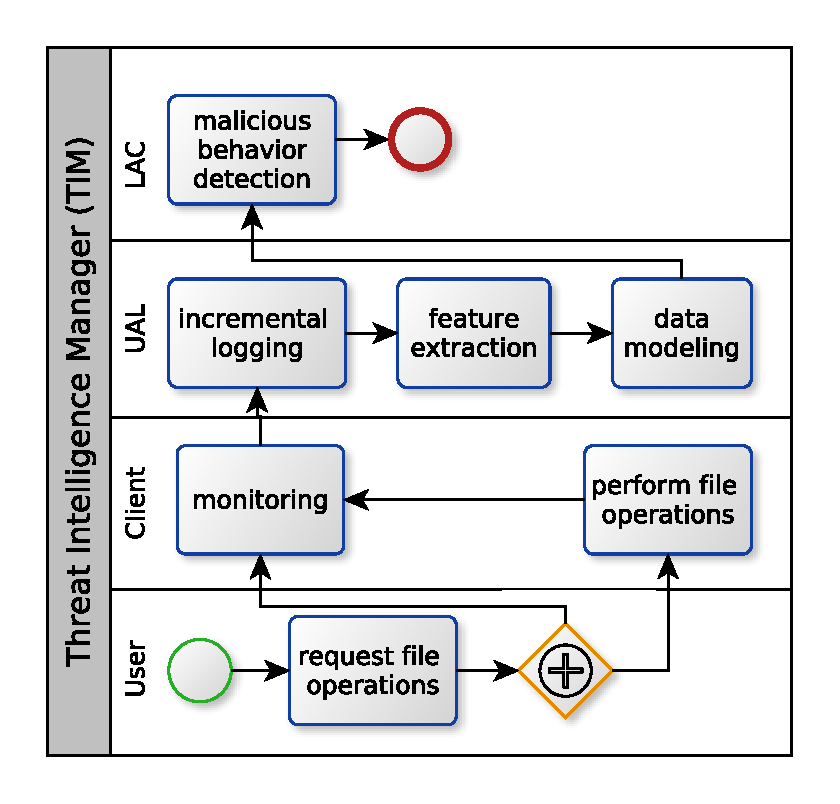
\includegraphics[width=10cm]{figs/ch3/fig06.eps}
	\caption{The Threat Intelligence Manager Workflow}
	\label{fig:3_06}
\end{figure}

As depicted in Figure \ref{fig:3_06}, users request operations are logged so that the main features can be monitored in the mobile client. The user behavior, trying or effectively executing operations, shall be incrementally captured and logged, making possible to monitor the main features that can reveal malicious behaviors, as well as to identify unexpected behaviors that can reveal possible threats. Therefore, the user operations are monitored by the client app, which sends the information to the User Activity Logging (UAL). 

The UAL is responsible for the incremental logging of activities of the mobile client, feature extraction and data modeling for malicious behavior detection, through the Log Analysis Center (LAC). As an internal module of the mobile client, the UAL implements monitors of selected events of the application, such as a login attempt or a file decryption, and logs the desired information for further analysis. The logged information shall be decomposed into selected features and modeled as matrices, composed of the number of occurrences of the selected features by its location and by time. The resultant data is submitted to the LAC, for anomaly detection.

The LAC performs the behavioral analysis through eigenvalue analysis and MOS schemes proposed by Eigensim, which identify anomalies on sparse, subtle or abrupt number of user operations. The malicious behavior detection is detail described in \ref{sec:3_eigensim}.

\section{Eigensim for Threat Intelligence}
\label{sec:3_eigensim}
In the context of anomaly-based schemes for attack detection, the proposed behavioral analysis approach applies signal processing techniques, such as subspace learning by eigenvalue decomposition and Model Order Selection schemes \cite{tenorio2013greatest}, for automatic detection of attacks or malicious behaviors. Model Order Selection is an effective signal processing technique for several applications, allowing separating the only noise components from the principal components applying a rank reduction of the data. 

Applying MOS to the analysis of user operations can be effective in order to reveal the occurrence of malicious behavior during an offline session. MOS for threat intelligence requires that the target features, such as user operations, should be modeled as a matrix composed by the number of occurrences grouped by location and time, and splited into $Q$ time frames. Therefore, the framework considers the time variations of the matrix $\pmb{X}^{(q)} \in \mathbb{R}^{M\times{N}}$, with $q = 1, \ldots, Q$, in order to detect the occurrence of malicious behaviors. For example, one element of $\pmb{X}^{(q)}$ can represent the number of file readings on folder $m$ during the minute $n$, from file operations logged by the mobile client.

The Eigensim can rely on sample covariance of zero mean variables (called as \pmb{zero mean covariance} for the sake of simplicity) and sample covariance of zero mean and unitary standard deviation (called as \pmb{zero mean and standardized covariance} for the sake of simplicity) variables, where the former is useful to identify abnormalities caused by large amounts of operations during a period, while the latter is applied to identify anomalies on sparse or subtle number of file operations.

Classical approaches to model order selection require the computation of the sample covariance matrix $\hat{\pmb{R}}_{yy}^{(q)}$ and of its eigenvalues, obtained from the measurement matrix $\pmb{X}$ of the zero mean samples given by

\begin{equation}\label{eq:3.03}
	\pmb{y}_{m}^{(q)} = \pmb{x}_{m}^{(q)} - \bar{\pmb{x}}_{m}^{(q)}.
\end{equation}

The set of obtained vectors $\pmb{y}_{m}^{(q)}$ composes the zero mean matrix $\pmb{Y}^{(q)}$, then the zero mean covariance matrix $\hat{\pmb{R}}_{yy}^{(q)}$ can be estimated as follows

\begin{equation}\label{eq:3.04}
	\hat{\pmb{R}}_{yy}^{(q)} = \frac{1}{N}\pmb{Y}^{(q)}\pmb{Y}^{(q)^{\rm T}},
\end{equation}
where $\hat{\pmb{R}}_{yy}^{(q)}$ means the estimation of the sample covariance matrix from the measured zero mean matrix $\pmb{Y}^{(q)}$ over $N$ minutes of the time frame $q$. 

For Eigensim based on sample covariance of zero mean and unitary standard deviation, in order to identify anomalies with sparse or subtle behavior, it is required, for each variable, to make the standard deviation unitary as follows

\begin{equation}\label{eq:3.05}
	\pmb{z}_{m}^{(q)} = \frac{\pmb{x}_{m}^{(q)} - \bar{\pmb{x}}_{m}^{(q)}}{\pmb{\sigma}_{m}^{(q)}}.
\end{equation}

The set of vectors $\pmb{z}_{m}^{(q)}$ composes the matrix $\pmb{Z}^{(q)}$, then the zero mean and standardized covariance matrix $\hat{\pmb{R}}_{zz}^{(q)}$ can be calculated via 

\begin{equation}\label{eq:3.06}
	\hat{\pmb{R}}_{zz}^{(q)} = \frac{1}{N}\pmb{Z}^{(q)}\pmb{Z}^{(q)^{\rm T}}.
\end{equation}

Once the $\hat{\pmb{R}}_{yy}$ or $\hat{\pmb{R}}_{zz}$ have been obtained for anomaly detection based on Eigensim, for the sake of simplicity, we refer to $\hat{\pmb{R}}_{yy}$ or $\hat{\pmb{R}}_{zz}$ as a matrix $\hat{\pmb{R}}$. Therefore, the next step of the algorithm is the eigenvalue decomposition (EVD), calculated according to $\hat{\pmb{R}}^{(q)} = \pmb{V}^{(q)}\pmb{\lambda}^{(q)}\pmb{V}^{(q)^{\rm T}}$, in order to obtain the vector of eigenvalues $\pmb{e}$, as following:

\begin{equation}\label{eq:3.07}
	\pmb{e}^{(q)} = \rm diag(\pmb{\lambda}^{(q)}),
\end{equation}

The eigenvalues should be sorted in descending order, as defined by $\lambda_{1}^{(q)} > \lambda_{2}^{(q)} > \lambda_{3}^{(q)} > \cdots > \lambda_{m}^{(q)}$, to make possible the selection of the first eigenvalue in the obtained sequence, represented by $\lambda_{1}^{(q)}$, which is the largest eigenvalue of the data evaluated for attack detection.

The process of obtaining the $\pmb{X}^{(q)} \in \mathbb{R}^{M\times{N}}$ and the matrix $\hat{\pmb{R}}^{(q)}$, finding the largest eigenvalue for each $q$-th time frame, should be repeated until $q = Q$, in order to obtain the largest eigenvalue of all time frames, as presented by 

\begin{equation}\label{eq:3.08}
	\pmb{E} =
	\begin{bmatrix}
		\lambda_1^{(1)} & \lambda_1^{(2)} & \lambda_1^{(3)} & \cdots & \lambda_1^{(Q)} \\
		\lambda_2^{(1)} & \lambda_2^{(2)} & \lambda_2^{(3)} & \cdots & \lambda_2^{(Q)} \\
		\lambda_3^{(1)} & \lambda_3^{(2)} & \lambda_3^{(3)} & \cdots & \lambda_3^{(Q)} \\
		\vdots & \vdots & \ddots & \vdots  \\
		\lambda_m^{(1)} & \lambda_m^{(2)} & \lambda_m^{(3)} & \cdots & \lambda_m^{(Q)} \\
	\end{bmatrix}.
\end{equation}

Since $\lambda_1^{(q)} > \lambda_2^{(q)} > \lambda_3^{(q)} > \cdots > \lambda_{m-1}^{(q)} > \lambda_m^{(q)}$, then the first line of the matrix $\pmb{E}$ contains the largest eigenvalues of each $q$-th time frame, which is the expected input for MOS schemes and can be expressed as 
\begin{equation}\label{eq:3.09}
	\pmb{e}_{\rm max} = [ \lambda_1^{(1)}, \lambda_1^{(2)} \cdots \lambda_1^{(Q)}]
\end{equation}

Once obtained the largest eigenvalues of each $q$-th time frame, it is possible to apply a selected MOS scheme to estimate the model order $\hat{d}$, which is the estimated number of time frames with malicious behavior. Therefore, $\pmb{e}_{\rm max}$ is used as input parameter for MOS schemes, according to the equation

\begin{equation}\label{eq:3.10}
	\hat{d} = \textrm{MOS}(\pmb{e}_{\rm max})
\end{equation}

Note that some MOS schemes may also require the amount of time that compose a time frame, such as $\hat{d} = \textrm{MOS}(\pmb{e}_{\rm max}, M)$. For more information about MOS schemes, interested readers are referred to Appendix \ref{apx:a_mos} and to \cite{da2009comparison}.

\section{Results and analysis}
\label{sec:3_results}

This section provides the detailed analysis of the results from the proposed approach regarding security and performance analysis.

\subsection{Security analysis}
\label{sec:3_sec_analysis}
The security analysis of the proposed model was performed from the user behavioral analysis. Two common attack scenarios were analyzed. First, the malicious outsider trying to infect or steal the important files. Second, the malicious expired user trying to steal the important files. 

\subsubsection{Common threat scenarios}
\label{sec:3_common}
This section provides the detailed description of the common scenarios in which the log and behavioral analysis is provided. The behavioral analysis can help to keep the user or administrator informed of the threat and take actions, as well as it can be useful in order to implement threat preventions or reactive actions to avoid threat propagation.

\begin{thm}
	An attacker uses a valid password to perform operations on a bulk of files.
\end{thm}

The session time defines the period when operations can be performed until the next session renewing. During this period, it is still necessary to identify attacks and malicious behavior on file operations, in order to avoid fast attacks to perform unauthorized access to information or data modification. Some attacks present behavioral patterns based on abrupt number of operations, such as the ransomware attack, which is a growing attack \cite{McAfee2015} that blocks the access to valuable resources and requires a payment in order to unblock the content. The access to the resources can be blocked by the attacker through some techniques, when the content is encrypted by the attacker, the ransomware attack can be called cryptoransomware or cryptolocker \cite{kaspersky2014}.

The Eigensim and MOS schemes based on zero mean covariance analysis are effective to reveal abrupt changing of behaviors over time \cite{tenorio2013greatest}, making possible to identify intense malicious behaviors on offline mode of mobile clients, such in case of ransomware attack or bulk access to sensitive data.

The large number of operations over time is a well-known pattern of some attacks, due to the efforts on security measures to make the attacks infeasible over time. In this context, the operations can also be evaluated in contrast to the estimated required time for operations done by legitimate behaviors, such as the evaluation of the mean time between operations, highlighting the occurrence of infeasible behaviors in comparison to legitimate user activities.

Sparse or subtle file operations, with low number of operations distributed over different files or directories, during short period of time can indicate anomalies in contrast to the required time for legitimate directory navigation. Eigensim and zero mean and standardized covariance analysis can be suitable if applied to evaluate the time and location of operations, in order to identify unreachable navigation, if compared to legitimate navigation

The Eigensim based on zero mean covariance analysis indicates abnormalities caused by large amounts of operations during a period. Subsequently, the eigenvalue analysis highlights massive or concentrated operations over time or folder location, which is evaluated by MOS schemes in order to identify the number of malicious behaviors during the evaluated time.

This threat scenario, where an attacker uses a valid password and session to perform operations on a bulk of files, can have its steps described as:

\begin{enumerate}[label=(\alph*)]
	\item The hacker has access to the mobile client and is able to perform operations;
	\item The session time is valid;
	\item The hacker tries to perform legitimate operations, such as file decryption, encryption, reading, writing or directory navigations;
	\item The mobile client incrementally append each operation attempt time into the logging;
	\item The TIM module evaluates the logging of legitimate operations, applying zero mean and standardized covariance analysis to identify anomalies on sparse or subtle number of file operations, highlighting the occurrence of infeasible behaviors in comparison to legitimate user activities;
	\item The TIM module evaluates the logging of legitimate operations, applying zero mean covariance analysis to identify abnormalities caused by massive operations during the session time.
\end{enumerate}

\begin{thm}
	Usage of expired password to perform unauthorized operations.
\end{thm}

In the offline mode, the session time is used to restrict the operations during a specified period, although it is possible to manipulate the current time in mobile device, to emulate a period in which the session was valid. The log analysis by Eigensim can deal with this kind of threat, through the incremental logging of the time when each operation was performed, followed by the behavioral evaluation of operations over time. 

The incremental logging assumes that new logged operations shall have equal or bigger time than the last logged operation, the violation of this rule means that the system is out of sync and indicates a malicious behavior. Additionally, a large amount or sparse operation performed at the same time, or during a short period, can indicate the use of backtrack techniques to maintain a valid session during necessary time to perform an attack. Massive, subtle or sparse malicious operation performed during a valid session time can be identified by MOS schemes based on covariance analysis.

Applying Eigensim to the analysis of the time between user operations can be effective in order to reveal the occurrence of malicious behavior during an offline session. The MOS based on zero mean and standardized covariance analysis identifies anomalies on sparse or subtle variation in the number of file operations, since the eigenvalue analysis highlights the unexpected number of sparse (such as file operations on diverse folders) or subtle operations. Consequently, the result of the eigenvalue analysis is applied to MOS schemes, in order to identify the occurrence of malicious behaviors during the valid session.

The Eigensim based on zero mean covariance analysis indicates abnormalities caused by large amounts of operations during a period. The eigenvalue analysis based on the zero mean covariance matrix highlights massive or concentrated operations over time or location, which is evaluated by MOS schemes in order to identify the number of malicious behaviors during the evaluated time.

This threat scenario, where the attacker uses expired password to perform unauthorized operations, can have its steps described as:

\begin{enumerate}[label=(\alph*)]
	\item The hacker steals the operating system;
	\item The hacker modifies the time of the operating system to a period when the session was valid;
	\item The hacker has access to the mobile client and is able to perform operations;
	\item The hacker tries to perform legitimate operations, such as file decryption, encryption, reading, writing or directory navigations;
	\item The mobile client incrementally append each operation attempt time into the logging;
	\item The mobile client verifies if one logged time is older than the last operation time. If it is true, the Eigensim module classifies the evaluated operation as malicious;
	\item The TIM module evaluates the logging of legitimate operations, applying zero mean and standardized covariance analysis to identify anomalies on sparse or subtle number of file operations;
	\item The TIM module evaluates the logging of legitimate operations, applying zero mean covariance analysis to identify abnormalities caused by massive operations during the session time;
\end{enumerate}

\subsubsection{Data Modeling for Behavioral Analysis }
\label{sec:3_data}

The Eigensim and MOS schemes are used in order to identify anomalous behavior that can indicate an attack and be used to prevent or avoid attack propagation. Therefore, it is necessary to analyze the data that can be collected from user operations on mobile client, to identify features that can be modeled and submitted to Eigensim, according to described in Section \ref{sec:3_eigensim}.

The selected features shall be modeled as matrices which represents a signal superposition of signal, artifact and noise, which refer to normal, controlled and anomalous behaviors \cite{tenorio2013greatest,vieira2017model}. Thus, the data is grouped into time frames $\pmb{X}^{(q)} \in \mathbb{R}^{M\times{N}}$, with $q = 1, 2, 3, \ldots, Q$ , where $M$ defines the decomposition of a selected feature, $N$ defines the time decomposition and represents the number of occurrences of the feature $m$ during the time $n$.

In offline mode, the user is still allowed to get access to operations that do not require communication with the server side. These operations and their selected features shall be incrementally logged by the UAL of the mobile client, in order to be analyzed by the TIM to identify malicious behaviors. 

This work proposes to evaluate the following features, which represents events of the user operating the mobile client.

\paragraph{\textbf{File Access (Time and File System Location)},}i.e. data access to selected files in offline mode, accessing the data stored on the mobile client. The file access feature can be decomposed into more detailed features, which are:

\begin{enumerate}
	\item number of file decryption;
	\item number of decrypted file reading;
	\item number of decrypted file execution. 
\end{enumerate}

Therefore, it is necessary to generate three matrices for the following malicious behaviors analysis: 

\begin{enumerate}[label=(\alph*)]
	\item massive file access, which can reveal data leakage and be identified by MOS schemes based on zero mean covariance analysis; 
	\item low file access into several folders, characterized by sparse operations that can reveal unreachable navigation performed by automated file accesses in order to avoid the massive file access characterization;
	\item Malicious sparse file accesses can be identified by MOS schemes based on zero mean and standardized covariance analysis. 
\end{enumerate}

\paragraph{\textbf{File Update (Time and File System Location)},}i.e. writing operations into selected files in offline mode, writing the data stored on the mobile client. The update feature can be decomposed into:

\begin{enumerate}
	\item number of file encryption;
	\item number of decrypted file writing.
\end{enumerate}

Therefore, it is necessary to generate two matrices for malicious behaviors analysis, such as: 

\begin{enumerate}[label=(\alph*)]
	\item massive file update, which can reveal ransomware or similar attacks and be identified by MOS schemes based on zero mean covariance analysis; 
	\item low number of file update into several folders, characterized by sparse operations that can reveal unreachable navigation performed by automated file accesses in order to avoid the massive file access characterization. Malicious sparse file accesses can be identified by MOS schemes based on zero mean and standardized covariance analysis.
\end{enumerate}

\paragraph{\textbf{File Download (Start Time, End Time and File System Location)},}i.e. download requests in online mode, evaluated by the mobile client. The file download feature shall be modeled as the matrix of number downloads by file location over time, in order to perform malicious behaviors analysis, such as:

\begin{enumerate}
	\item massive data leakage or similar attacks, which can be identified by MOS schemes based on zero mean covariance analysis;
	\item low number of file download from several folders, characterized by sparse operations, which can reveal unreachable navigation performed by automated file download in order to avoid the massive file download characterization. Malicious sparse file download can be identified by MOS schemes based on zero mean and standardized covariance analysis.
\end{enumerate}

\paragraph{\textbf{File Upload (Start Time, End Time and File System Location)},}i.e. upload requests in online mode, evaluated by the mobile client. The file upload feature can reveal attempts of ransomware or similar attacks and be identified by MOS schemes based on covariance analysis. Therefore, it is necessary model the matrix of number uploads by file location over time, in order to perform malicious behaviors analysis, such as:

\begin{enumerate}
	\item massive file upload, similar to ransomware attack, which can be identified by MOS schemes based on zero mean covariance analysis; 
	\item low number of file upload to several folders, characterized by sparse operations, which can reveal unreachable navigation performed by automated file upload in order to avoid the massive file upload characterization. Malicious sparse file upload can be identified by MOS schemes based on zero mean and standardized covariance analysis.
\end{enumerate}

\subsection{Performance analysis}
\label{sec:3_complex}

The proposed concept of mobile client security has been implemented in the Storgrid protected cloud environment \cite{storgrid2016}. Therefore, the approach is correlated with the practical usability requirements: the corporate user continues to use the mobile storage app in offline and does not need to reload the files every time the key is renewed. This methodology can be used in other mobile clients. The common advantage is that the mobile client performs the operations both in the offline and online mode and uses the key expiry to protect the privacy of the corporate data. 

The log analysis of the Log Analysis Center (LAC) has been implemented and evaluated for offline anomaly detection in mobile clients, making it possible to apply anomaly detection techniques in a lightweight fashion, considering low processing requirements for deal with the resource constraints of mobile clients. The evaluation considered the required processing time for anomaly detection from log analysis, measuring the data modeling time through the UAL, the eigenvalue decomposition time and the required time for the EDC MOS scheme execution, which is the scheme that requires less processing capacity and provides more anomaly identification accuracy \cite{da2009comparison,tenorio2013greatest}. 

The experiments were performed in two mobile devices, Galaxy GT-I9300 and Galaxy Tab SM-T800, with variations of log size and window size. The Galaxy GT-I9300 has Quad-core 1.4 GHz Cortex-A9 processor and 1 GB RAM, while the Galaxy Tab SM-T800 has its processing capacity composed by Quad-core 1.9 GHz Cortex-A15 and quad-core 1.3 GHz Cortex-A7, and 3 GB RAM.

Table \ref{tab:3_04} presents the data modeling time and the processing time of eigenvalues decomposition calculations to be applied to anomaly detection from user operation logs of Storgrid mobile client. 

\begin{table*}
	\caption{Data Modeling and Eigenvalue Decomposition Time}
	\scriptsize
	\label{tab:3_04}
	\centering
	\begin{tabular}{|l|l|l|l|l|l|l|l|}
		\hline \rowcolor{Gray} Device	& \begin{tabular}[x]{@{}l@{}}Log Size\\(MB)\end{tabular}	& \begin{tabular}[x]{@{}l@{}}Window\\(min)\end{tabular}	& \begin{tabular}[x]{@{}l@{}}Modeling\\(ms)\end{tabular}	& \begin{tabular}[x]{@{}l@{}}Avg. Eig.\\(ms)\end{tabular}	& \begin{tabular}[x]{@{}l@{}}Std. Eig.\\(ms)\end{tabular}	& \begin{tabular}[x]{@{}l@{}}Eig. Min.\\(ms)\end{tabular}	& \begin{tabular}[x]{@{}l@{}}Eig. Max.\\(ms)\end{tabular}	\\ \hline
		Galaxy GT-I9300	& 6	& 60	& 107	& 209.52	& 18.58	& 183	& 276	\\ \hline
		Galaxy GT-I9300	& 6	& 40	& 115	& 227.26	& 18.13	& 191	& 289	\\ \hline
		Galaxy GT-I9300	& 6	& 20	& 89	& 268.14	& 21.94	& 229	& 315	\\ \hline
		Galaxy GT-I9300	& 6	& 10	& 90	& 347.42	& 24.11	& 304	& 421	\\ \hline
		Galaxy GT-I9300	& 4.1	& 60	& 20	& 60.90	& 15.19	& 37	& 106	\\ \hline
		Galaxy GT-I9300	& 4.1	& 40	& 20	& 68.72	& 15.71	& 43	& 114	\\ \hline
		Galaxy GT-I9300	& 4.1	& 20	& 34	& 89.04	& 16.78	& 54	& 133	\\ \hline
		Galaxy GT-I9300	& 4.1	& 10	& 21	& 117.24	& 14.36	& 96	& 171	\\ \hline
		Galaxy GT-I9300	& 1.4	& 60	& 10	& 159.82	& 15.82	& 125	& 197	\\ \hline
		Galaxy GT-I9300	& 1.4	& 40	& 10	& 168.06	& 15.90	& 139	& 220	\\ \hline
		Galaxy GT-I9300	& 1.4	& 20	& 11	& 204.4	& 20.46	& 176	& 269	\\ \hline
		Galaxy GT-I9300	& 1.4	& 10	& 13	& 259.00	& 21.34	& 220	& 315	\\ \hline
		Galaxy Tab SM-T800	& 6	& 60	& 7	& 59.30	& 6.55	& 54	& 74	\\ \hline
		Galaxy Tab SM-T800	& 6	& 40	& 8	& 62.56	& 7.05	& 56	& 80	\\ \hline
		Galaxy Tab SM-T800	& 6	& 20	& 10	& 73.28	& 8.59	& 65	& 95	\\ \hline
		Galaxy Tab SM-T800	& 6	& 10	& 8	& 93.48	& 9.13	& 83	& 130	\\ \hline
		Galaxy Tab SM-T800	& 4.1	& 60	& 11	& 18.64	& 4.51	& 16	& 38	\\ \hline
		Galaxy Tab SM-T800	& 4.1	& 40	& 11	& 19.64	& 5.12	& 17	& 38	\\ \hline
		Galaxy Tab SM-T800	& 4.1	& 20	& 12	& 25.12	& 5.55	& 21	& 46	\\ \hline
		Galaxy Tab SM-T800	& 4.1	& 10	& 12	& 32.32	& 7.29	& 27	& 55	\\ \hline
		Galaxy Tab SM-T800	& 1.4	& 60	& 4	& 49.08	& 6.01	& 42	& 62	\\ \hline
		Galaxy Tab SM-T800	& 1.4	& 40	& 5	& 51.42	& 7.36	& 44	& 74	\\ \hline
		Galaxy Tab SM-T800	& 1.4	& 20	& 5	& 51.12	& 7.80	& 54	& 91	\\ \hline
		Galaxy Tab SM-T800	& 1.4	& 10	& 7	& 75.24	& 7.71	& 65	& 90	\\ \hline
	\end{tabular}
\end{table*}

The information presented by column are the device model, the log size in megabytes, the window size in minutes, the data modeling time in milliseconds, the average of eigenvalue decomposition time in milliseconds, the standard deviation of eigenvalue decomposition time in milliseconds, the minimum of eigenvalue decomposition time in milliseconds and the maximum of eigenvalue decomposition time in milliseconds.

The results show that the lower window size leads to the larger eigenvalue decomposition time, but the largest eigenvalue decomposition time, which was the maximum of 421 milliseconds with average of 347.42 milliseconds. This result highlights an acceptable speed even for the worst evaluated scenario, which is the case using a Galaxy GT-I9300 for processing 6MB with window size of 10 minutes.

\begin{table*}[!t]
	\caption{EDC MOS scheme processing time for anomaly detection}
	\footnotesize
	\label{tab:3_05}
	\centering
	\begin{tabular}{|l|l|l|l|l|l|l|l|}
		\hline \rowcolor{Gray} Device	& \begin{tabular}[x]{@{}l@{}}Log Size\\(MB)\end{tabular}	& \begin{tabular}[x]{@{}l@{}}Window\\(min)\end{tabular}	& \begin{tabular}[x]{@{}l@{}}Avg. EDC.\\(ms)\end{tabular}	& \begin{tabular}[x]{@{}l@{}}Std. EDC.\\(ms)\end{tabular}	& \begin{tabular}[x]{@{}l@{}}Min. EDC.\\(ms)\end{tabular}	& \begin{tabular}[x]{@{}l@{}}Max. EDC.\\(ms)\end{tabular}	\\ \hline
		Galaxy GT-I9300	& 6	& 60	& 5.27	& 4.04	& 3	& 20	\\ \hline
		Galaxy GT-I9300	& 6	& 40	& 10.78	& 6.37	& 6	& 34	\\ \hline
		Galaxy GT-I9300	& 6	& 20	& 32.62	& 12.44	& 21	& 88	\\ \hline
		Galaxy GT-I9300	& 6	& 10	& 115.08	& 17.45	& 88	& 158	\\ \hline
		Galaxy GT-I9300	& 4.1	& 60	& 5.68	& 4.18	& 3	& 23	\\ \hline
		Galaxy GT-I9300	& 4.1	& 40	& 10.76	& 5.31	& 7	& 27	\\ \hline
		Galaxy GT-I9300	& 4.1	& 20	& 37.58	& 10.30	& 23	& 61	\\ \hline
		Galaxy GT-I9300	& 4.1	& 10	& 125.98	& 18.56	& 101	& 191	\\ \hline
		Galaxy GT-I9300	& 1.4	& 60	& 4.92	& 3.49	& 3	& 17	\\ \hline
		Galaxy GT-I9300	& 1.4	& 40	& 9.00	& 4.23	& 6	& 25	\\ \hline
		Galaxy GT-I9300	& 1.4	& 20	& 30.14	& 9.21	& 19	& 62	\\ \hline
		Galaxy GT-I9300	& 1.4	& 10	& 100.62	& 15.83	& 69	& 163	\\ \hline
		Galaxy Tab SM-T800	& 6	& 60	& 1.84	& 0.65	& 1	& 3	\\ \hline
		Galaxy Tab SM-T800	& 6	& 40	& 3.26	& 1.24	& 2	& 7	\\ \hline
		Galaxy Tab SM-T800	& 6	& 20	& 10.90	& 2.40	& 9	& 21	\\ \hline
		Galaxy Tab SM-T800	& 6	& 10	& 41.86	& 7.33	& 34	& 60	\\ \hline
		Galaxy Tab SM-T800	& 4.1	& 60	& 1.85	& 0.60	& 1	& 3	\\ \hline
		Galaxy Tab SM-T800	& 4.1	& 40	& 3.62	& 1.10	& 2	& 8	\\ \hline
		Galaxy Tab SM-T800	& 4.1	& 20	& 12.04	& 2.79	& 9	& 22	\\ \hline
		Galaxy Tab SM-T800	& 4.1	& 10	& 40.16	& 6.48	& 35	& 60	\\ \hline
		Galaxy Tab SM-T800	& 1.4	& 60	& 1.98	& 0.89	& 1	& 6	\\ \hline
		Galaxy Tab SM-T800	& 1.4	& 40	& 3.30	& 1.16	& 2	& 7	\\ \hline
		Galaxy Tab SM-T800	& 1.4	& 20	& 10.48	& 2.90	& 8	& 21	\\ \hline
		Galaxy Tab SM-T800	& 1.4	& 10	& 34.52	& 4.08	& 30	& 45	\\ \hline
	\end{tabular}
\end{table*}

Table \ref{tab:3_05} presents the processing time of EDC MOS calculations applied to anomaly detection from user operation logs of Storgrid mobile client. Table \ref{tab:3_05} respectively presents the device model, the log size in megabytes, the window size in minutes, the average of EDC calculation time in milliseconds, the standard deviation of EDC calculation time in milliseconds, the minimum of EDC calculation time in milliseconds and the maximum of EDC calculation time in milliseconds.

It is possible to observe that the processing time increases with the window size decreasing, similar to the results for eigenvalue decomposition time. The longest processing time measured is lower than 200 milliseconds, even considering window size of 10 minutes or processing 6 MB of user operation log. This result represents an acceptable processing time for anomaly detection in mobile clients.

\section{Conclusion and future work}
\label{sec:3_conclusion}

An important security issue faced by corporations that use cloud-based systems is how to provide security mechanisms to support offline corporate mobile clients. Once a mobile client releases the connection with the corporate cloud, no security measure implemented in the cloud infrastructure assures the protection of sensitive data stored in the mobile device. Aware of this problem and its importance, this work presented a proposal to address the offline mobile security problem combining cryptographic methods and a Eigensim-based behavioral anomaly detection. 

As prove of concept, a fully working mobile application was developed to test the proposed security solution and acquired results provide evidence that besides achieving the desired security features, the solution also has positive results in terms of performance. This fact is due to the usage of lightweight operations and the optimized combination of the selected security methods. The proposed approach is a practical application to be used in the corporate mobile environment. It is implemented as a fully working mobile client and can be used for any type of enterprise. Also, part of concept is seed for new security solutions for big data apps. 
